\chapter{群论}
\section{基本定义}
\begin{definition}[群]
    (1) 封闭性 (2) 结合律 (3) 单位元 (4) 逆元
\end{definition}
\begin{definition}[有限群]
    若群$G$有限, 则其成员个数$|G|$称为阶数。
\end{definition}
\begin{definition}[Abel群]
    运算\colorbf{可交换}的群, 如整数模$n$的加法群$\mathbb{Z}_n$。
\end{definition}
\begin{definition}[阶数]
    若$g\in G$, 使得$g^r=e$的最小正整数$r\in\mathbb{Z}_{>0}$称为其阶数。
\end{definition}
\begin{definition}[子群]
    $H\leq G$是指$H\subset G$且$H$在$G$运算下构成群。容易看出单位元$e\in G$。
\end{definition}
\begin{exercise}[教材B.1]
    证明有限群的成员都有阶数, 即$\forall g\in\text{有限群}, \exists r\in\mathbb{Z}_{>0},\st g^r=e$。
\end{exercise}
\begin{proof}
    若某个成员$g$没有阶数, 则群$G$有无限大的子集$\qty{g^r:r\in\mathbb{Z}_{>0}}$, 矛盾。进一步, 我们知道群$G$的任何成员的阶数不超过$|G|$。
\end{proof}
\begin{exercise}[教材B.2, Lagrange定理]
    若$H\leq\text{有限群$G$}$, 则$|H|$可整除$|G|$, 除数$[G:H]=\frac{|G|}{|H|}$称为子群$H$的\sffamily{Lagrange指数}。
\end{exercise}
\par 为了证明此定理我们需要引入一些概念:
\begin{definition}[陪集]
    设$H\leq g$, 集合$gH=\qty{gh:h\in H}$, $Hg=\qty{hg:h\in H}$称为$g$对$H$的\colorbf{左陪集}和\colorbf{右陪集}。
\end{definition}
\begin{proposition}
    $gH=H\Longleftrightarrow g\in H$
\end{proposition}
\begin{proof}
    $g\in H\Longrightarrow gH=H$是显然的, 反过来时注意到$e\in H$, 则$g=ge\in gH=H$。
\end{proof}
\begin{proposition}
    $g_1H\cap g_2H=\begin{dcases}
        \text{非空集合} & (g_1H=g_2H)\\
        \varnothing & (g_1H\neq g_2H)
    \end{dcases}$
\end{proposition}
\begin{proof}
    对$\forall g\in g_1H$有$g=g_1h=g_2\qty(g_2^{-1}g_1h)\ (h\in H)$。若$\exists\text{成员$g$}\in g_1H\cap g_2H$, 则有$h_1,h_2\in H\st g=g_1h_1=g_2h_2$ $\Longrightarrow$ $g_2^{-1}g_1=h_2h_1^{-1}\in H$, 由此$g=g_2\qty(g_2^{-1}g_1h)\in g_2H$。类似的$\forall g\in g_2H$ $\Longrightarrow$ $g\in g_1H$, 这就证明了$g_1H=g_2 H$。
\end{proof}
\begin{proposition}
    全部陪集的并$\bigcup_{g\in G}gH=G$。
\end{proposition}
\begin{proof}
    \par 由$gH\subset G$可知$\bigcup_{g\in G}gH\subset G$。
    \par 另一方面, 由于$e\in H$, 故$\forall g\in G, g=ge\in gH$, 这说明$\forall g\in G:G\subset gH$ $\Longrightarrow$ $g\subset\bigcup_{g\in G}gH$。
    \par 综合上述所论, $\bigcup_{g\in G}gH\subset G\land g\subset\bigcup_{g\in G}gH$ $\Longrightarrow$ $G=\bigcup_{g\in G}gH$。
\end{proof}
\begin{proof}[教材习题B.2, Lagrange定理]
    我们知道全部陪集$\{gH:g\in G\}$是一组不交的集合, 容易看出$\bigcup$ $\{gH:g\in G\}=G$, 即$G=\bigsqcup\{gH:g\in G\}=\bigsqcup gH$, 这说明$|G|=\sum |gH|$。容易证明$|gH|=|H|$, 这说明$|G|=\sum |gH|=\sum |H|=|H|\sum 1$, 由此命题得证。
\end{proof}

\begin{exercise}[教材B.3]
    证明每个成员$g\in G$的阶数可以整除$|G|$。
\end{exercise}
\begin{proof}
    \par 令$H=\qty{g^r:1\leq r\leq r_k}=\qty{g,g^2,\cdots,g^{r_k-1},g^{r_k}=e}$, 则容易看出$H\leq G$, 根据Lagrange定理, $H$的指数$[G:H]=\frac{|G|}{|H|}\in\mathbb{Z}_{>0}$, 即$|G|=[G:H]\cdot |H|=[G:H] r_k$ $\Longrightarrow$ $r_k\mid |G|$。
\end{proof}

\begin{definition}
    若$\exists g\in G,\st\text{群成员$a,b\in G$满足$b=g^{-1}ag$}$, 则称$a,b$为共轭成员。
\end{definition}
\begin{proposition}
    群成员间的共轭是等价关系。
\end{proposition}
\begin{proof}
    \begin{enumerate}
        \item 任意成员$a$与其自身共轭:
        $$a=e^{-1}ae$$
        \item 若成员$a$与成员$b$共轭, 则成员$b$与成员$a$共轭:
        $$\qty(b=g^{-1}ag)\Longrightarrow\qty[a=\qty(g^{-1})^{-1}b\qty(g^{-1})]$$
        \item 若成员$a$与成员$b$共轭, 成员$b$与成员$c$共轭, 则成员$a$与成员$c$共轭:
        $$\qty(b=g^{-1}ag)\land\qty(c=g'^{-1}bg')\Longrightarrow\qty[c=g'^{-1}gagg'=\qty(gg')^{-1}a\qty(gg)]$$
    \end{enumerate}
\end{proof}
\begin{definition}[正规子群]
    若$H\leq G$且$\forall g\in G: g^{-1}Hg=H$ (或等价的$Hg=gH$), 则称$H$为$G$的\colorbf{正规子群}, 记作$H\unlhd G$, 记号$H\lhd G$表示$H\neq G$的正规子群。
\end{definition}
\par 我们指出, Abel群的任何子群都是正规子群。设$H\leq\text{Abel群$G$}$, 由于子群$H$的成员也是其继承的Abel群的成员, 这些成员与$G$中任意成员$g$也是可交换的, 故$Hg=gH$显然成立。
\par 对群$G$, $x\in G$的共轭类定义为$G_x\equiv\qty{g^{-1}xg:g\in G}$。容易看出$y\in G_x\Longrightarrow x\in G_y$。注意到
\[\begin{split}
    y\in G_x&\Longrightarrow \exists g\in G:y=g^{-1}xg\\
    &\Longrightarrow \exists g\in G: x=gyg^{-1}=\qty(g^{-1})^{-1}y\qty(g^{-1})\\
    &\xRightarrow{g^{-1}\in G} \exists g\in G: x=g^{-1}yg\Longrightarrow x\in G_y
\end{split}\]
\begin{exercise}[教材B.4]
    $y\in G_x\Longrightarrow G_y=G_x$
\end{exercise}
\begin{proof}
    由于$y\in G_x$, $\exists g_0\in G:y=g_0^{-1}xg_0$或$x=g_0yg_0^{-1}$。现在设$t\in G_y$, 即$\exists g\in G:t=g^{-1}yg=g^{-1}g_0^{-1}xg_0g=(g_0g)^{-1}x(g_0g)$ $\Longrightarrow$ $t\in G_x$, 这就证明了$G_y\subset G_x$。反过来设$t\in G_x$, 即$\exists g\in G:t=g^{-1}xg=g^{-1}g_0yg_0^{-1}g=\qty(g_0^{-1}g)^{-1}y\qty(g_0^{-1}g)$ $\Longrightarrow$ $t\in G_y$。这就证明了$G_x\subset G_y$。综合上述, 我们有$G_y=G_x$。
\end{proof}
\begin{exercise}[教材B.5]
    $x\in\text{Abel群$G$}\Longrightarrow G_x=\{x\}$
\end{exercise}
\begin{definition}[生成元]
    设$g_1,g_2,\cdots,g_\ell\in\text{群$G$}$, 则$G$中全部可以写成$g_1,g_2,\cdots,g_\ell$中若干个成员之乘积的群成员构成$G$的一个子集, 叫做$g_1,g_2,\cdots,g_\ell$所生成的子群$H$, 记作$H=\expval{g_1,g_2,\cdots,g_\ell}$, 即
    $$\expval{g_1,g_2,\cdots,g_\ell}=\qty{g_1^{n_1}g_2^{n_2}\cdots g_\ell^{n_\ell}=\prod_{k=1}^\ell g_k^{n_k}:(n_1,n_2,\cdots,n_\ell)\in\qty(\mathbb{Z}_{\geq 0})^\ell}$$
    $g_1,g_2,\cdots,g_\ell$称为子群$\expval{g_1,g_2,\cdots,g_\ell}$的生成元。
\end{definition}
\par 如果基群$G$是很大的或平凡的, 那么由给定成员生成的继承$G$的子群也称为($G$的)一个\colorbf{生成群}, 我们可以略去$G$的表述。容易看出生成一个阶数为$n$的生成群至少需要$\log(n)$个成员。
\begin{definition}[循环群]
    单个成员生成的生成群称为这个成员的\textbf{循环群}。容易看出循环群的阶数等于其生成元的阶数。
\end{definition}
\begin{exercise}[教材B.6]
    阶数为素数的群是循环群。
\end{exercise}
\par 为了证明此命题, 我们需要如下结论:
\begin{proposition}
    $\text{生成群的阶数等于其某个生成元的阶数}\Longleftrightarrow\text{此群为循环群}$
\end{proposition}
\begin{proof}
    $(\Longleftarrow)$是明显的, 现在来证明$(\Longrightarrow)$。设$G=\expval{g_1,g_2,\cdots,g_n}$, 其中$g_1$的阶数为$|G|$, 我们的目标是证明$G=\expval{g_1}$。明显$\expval{g_1}\subset\expval{g_1,g_2,\cdots,g_n}=G$, 我们注意到由于$g_1$的阶数为$|G|$, 则$\expval{g_1}$必然包含$e$, $g_1$, $g_1^2$, $\cdots$, $g_1^{|G|-1}$这$|G|$个不同的成员, 也就是说$\qty|\expval{g_1}|=|G|$, 这说明$\expval{g_1}=G$。
\end{proof}
\begin{proof}[教材习题B.6]
    若群$G$的阶数$|G|$为素数, 考虑继承$G$的子群$H\leq G$, 则根据Lagrange定理可知其阶数$|H|$应满足$|G|=[G:H]\cdot |H|$。由于$|G|$是素数, $H$的阶数和对基群$G$的指数均为整数, 那么必有$[G:H]=1, |H|=|G|$或$[G:H]=|G|, |H|=1$。若$[G:H]=1, |H|=|G|$, 则$H=G$是平凡情况, 另一种情况$[G:H]=|G|, |H|=1$, 这说明$H=\qty{e}$, 也就是说继承$G$的子群只有$\qty{e}$。对任何生成元个数$>1$的生成群, 其部分生成元单独生成的群都是继承此生成群的子群, 这说明$G$的生成元只有$1$个, 也就是说$G$是循环群。
\end{proof}
\par 值得注意的是, 循环群是可以有不平凡的子群的, 例如对4阶循环群$G=\langle e,g,g^2,g^3\rangle$, 子群$H=\langle e,g^2\rangle$就是继承$G$的子循环群, 可以看出$G=\langle g\rangle$, $H=\langle g^2\rangle$。仅阶数为素数的循环群才会只有平凡的子群, 因为素数是没有$1$和其自身以外的因子的。
\begin{exercise}[教材B.7]
    每个循环群的子群也是循环群。
\end{exercise}
\begin{proof}
    继承循环群的子群也能够表示成单个成员的次幂, 因而也是循环群。
\end{proof}
\begin{exercise}[教材B.8]
    若$g\in G$的阶数$r$有限, 则$g^m=g^n\Longleftrightarrow m=n\pmod r$
\end{exercise}
\begin{proof}
    $m=n\pmod r$说明存在$k_1,k_2\in\mathbb{Z}_{\geq 0}$以及余数$s=m\bmod r=n\bmod r\in\mathbb{Z}_{\geq 0}\cap\Ico{0,r}$, 使得$m=k_1r+s$, $n=k_2r+s$, 那么$g^m=g^{k_1r+s}=\qty(g^r)^{k_1}g^s=g^s$, 同理$g^n=g^s$, 这就证明了$(\Longleftarrow)$。
    \par 若$g^m=g^n$, 则$g^{m+(r-n)}=g^r=e$, 即$r\mid (m-n+r)$ $\Longrightarrow$ $r\mid (m-n)$, 也就是$m=n\pmod r$。
\end{proof}
\begin{exercise}[教材B.9]
    群$G$的成员$g_1,g_2$在继承$G$的同一个子群$H$的陪集中$\Longleftrightarrow$ $\exists h\in H$满足$g_2=g_1h$。
\end{exercise}
\begin{proof}
    $(\Longrightarrow)$是显然的, 现在来证$(\Longleftarrow)$。容易看出$g_2\in g_1H$, $g_1=g_2h^{-1}\in g_2H$。$\forall t\in g_1H:$ $\exists h_1\in H$, $\st t=g_1h_1=g_2h^{-1}h_1\in g_2H$, 这就证明了$g_1H\subset g_2H$。类似的可以证明$g_2H\subset g_1H$, 即$g_1H=g_2H$。
\end{proof}

\section{表示}
\par 一个$n$维矩阵群是一个$n\times n$矩阵构成的集合, 在矩阵乘法下构成群。为了方便我们用\texttt{mathcal}字母来表示矩阵群。我们记$F^{m\times n}=\qty{M_{m\times n}=[m_{ij}]_{m\times n}: m_{ij}\in F}$ ($F$为数域)。单位矩阵记作$I_n=[\delta_{ij}]_{n\times n}$, 我们已经规定了如下的矩阵群, 称为\colorbf{典型群}:
\begin{flalign*}
    &\qquad\text{\colorbf{一般线性群}}& &\begin{dcases}
        GL(n,F)=\qty{M_n\in F^{n\times n}:\det M_n\neq 0}&\\
        GL_+(n,F)=\qty{M_n\in F^{n\times n}:\det M_n>0},\quad GL_-(n,F)=\qty{M_n\in F^{n\times n}:\det M_n<0}
    \end{dcases}&\\[5pt]
    &\qquad\text{\colorbf{特殊线性群}}& &\begin{dcases}
        SL(n,F)=\qty{M_n\in F^{n\times n}:\qty|\det M_n|=1}&\\
        SL_+(n,F)=SL(n,F)\cap GL_+(n,F),\quad SL_-(n,F)=SL(n,F)\cap GL_-(n,F)
    \end{dcases}&\\[5pt]
    &\qquad\text{\colorbf{正交群}}& &\begin{dcases}
        O(n)=\qty{M_n\in\mathbb{R}^{n\times n}:M_n^\top M_n=I_n}&\\
        O_+(n)=O(n)\cap GL_+(n,\mathbb{R}),\quad O_-(n)=O(n)\cap GL_-(n,\mathbb{R})
    \end{dcases}&\\[5pt]
    &\qquad\text{\colorbf{特殊正交群}}& &\begin{dcases}
        SO(n)=O(n)\cap SL(n,\mathbb{R})&\\
        SO_+(n)=SO(n)\cap GL_+(n,\mathbb{R}),\quad SO_-(n)=SO(n)\cap GL_-(n,\mathbb{R})
    \end{dcases}&\\[5pt]
    &\qquad\text{\colorbf{幺正群}}& &\begin{dcases}
        U(n)=\qty{M_n\in\mathbb{C}^{n\times n}:M_n^\dagger M_n=I_n}&\\
        U_+(n)=O(n)\cap GL_+(n,\mathbb{C}),\quad U_-(n)=O(n)\cap GL_-(n,\mathbb{C})
    \end{dcases}&\\[5pt]
    &\qquad\text{\colorbf{特殊幺正群}}& &\begin{dcases}
        SU(n)=U(n)\cap SL(n,\mathbb{C})&\\
        SU_+(n)=SU(n)\cap GL_+(n,\mathbb{C}),\quad SU_-(n)=SU(n)\cap GL_-(n,\mathbb{C})
    \end{dcases}&
\end{flalign*}
\begin{definition}[表示]
    群$G$的\colorbf{表示}是一个保持群乘法的映射$\rho:G\to\text{矩阵群$\mathcal{G}$}$, 其\colorbf{维数}为矩阵群$\mathcal{G}$的维数, 记作$d_\rho$。单射表示称为\colorbf{同态表示}, 双射表示称为\colorbf{同构表示}。
\end{definition}
\par 我们知道矩阵对应线性映射, $n\times n$矩阵就对应着$n$维空间上的线性变换。如果我们变换空间的坐标系(将其基矢变换到另一组基矢), 那么在旧坐标系下表示这个线性变换的矩阵将变成一个新的矩阵。我们设旧坐标系下的基矢为$\vec{e}_1,\vec{e}_2,\cdots,\vec{e}_n$, 在线性变换下变成一组新的基矢$\vec{f}_1,\vec{f}_2,\cdots,\vec{f}_n$, 不妨设坐标的变换为
$$(x_1,x_2,\cdots,x_n)_{\vec{e}_1,\vec{e}_2,\cdots,\vec{e}_n}\longrightarrow(y_1,y_2,\cdots,y_n)_{\vec{f}_1,\vec{f}_2,\cdots,\vec{f}_n},\qquad y_i=\sum_{k=1}^n\lambda_{ik}x_k$$
为了搞清楚变换的本质, 我们在区别于 \textcolor{03468F}{$\vec{e}_1,\vec{e}_2,\cdots,\vec{e}_n$} 和 \textcolor{82218B}{$\vec{f}_1,\vec{f}_2,\cdots,\vec{f}_n$} 两组基矢以外的第三个固定坐标系下研究问题, 如 \ref{fig:coordinate_transfer} 所示。
\begin{figure}[htbp]
    \centering
    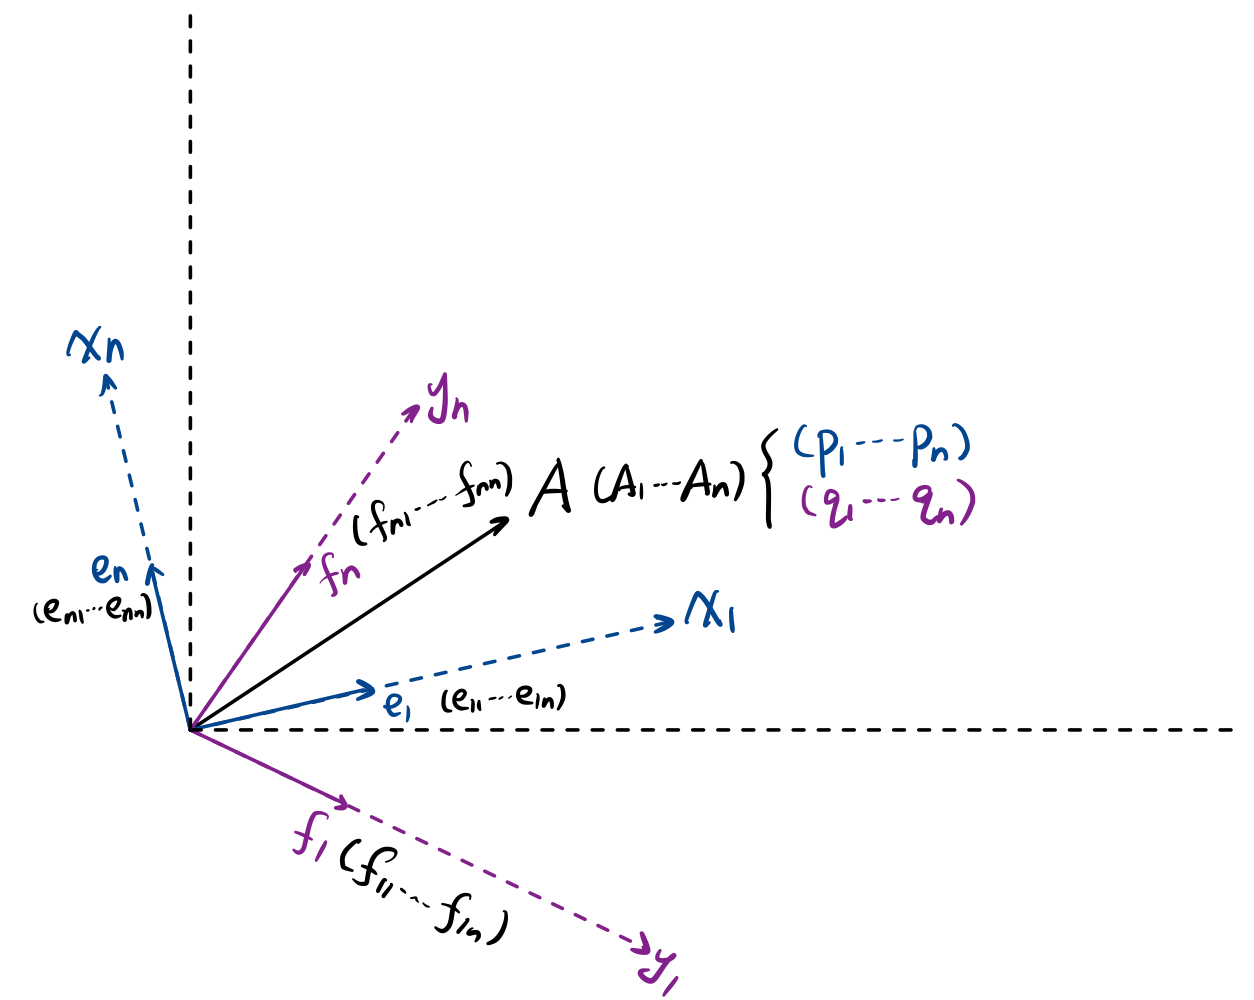
\includegraphics[width=.5\textwidth]{figures/coordinate_transfer.png}
    \caption{坐标系的变换}
    \label{fig:coordinate_transfer}
\end{figure}
设这两组基矢的坐标为$\vec{e}_k=(e_{k1},e_{k2},\cdots,e_{kn})$和$\vec{f}_i=(f_{i1},f_{i2},\cdots,f_{in})$ $(k,i=1,2,\cdots,n)$, 对一个固定的矢量$\vec{A}$我们有
$$\vec{A}=(p_1,p_2,\cdots,p_n)_{\vec{e}_1,\vec{e}_2,\cdots,\vec{e}_n}=(q_1,q_2,\cdots,q_n)_{\vec{f}_1,\vec{f}_2,\cdots,\vec{f}_n}$$
根据变换规律$q_i=\sum_{k=1}^n\lambda_{ik}p_k$, 我们显示写出$\vec{A}$的两组基底展开式
$$\vec{A}=\sum_{k=1}^n p_k\vec{e}_k=\sum_{i=1}^n q_i\vec{f}_i=\sum_{i=1}^n\qty(\sum_{k=1}^n\lambda_{ik}p_k)\vec{f}_i=\sum_{i=1}^n\sum_{k=1}^n\lambda_{ik}p_k\vec{f}_i$$
上式给出了系数$\lambda_{ik}$的意义: 这个系数同时可以用作坐标的变换和基矢的变换:
$$\vec{e}_k=\sum_{i=1}^n\lambda_{ik}\vec{f}_i,\qquad\text{或}\quad q_i=\sum_{k=1}^n\lambda_{ik}p_k$$
我们将其写成矩阵的形式, 为此引入记号:
$$x=\mqty[p_1\\p_2\\ \vdots\\ p_n],\quad y=\mqty[q_1\\q_2\\ \vdots\\ q_n],\quad E=\mqty[e_{11}& e_{21}& \cdots& e_{n1}\\ e_{12}& e_{22}& \cdots& e_{n2}\\ \vdots&\vdots&&\vdots\\ e_{1n}& e_{2n}& \cdots& e_{nn}],\quad F=\mqty[f_{11}& f_{21}& \cdots& f_{n1}\\ f_{12}& f_{22}& \cdots& f_{n2}\\ \vdots&\vdots&&\vdots\\ f_{1n}& f_{2n}& \cdots& f_{nn}]\ \footnote{这里矩阵$E,F$的矩阵元貌似进行了转置, 这是因为我们想要把$E,F$写成$E=(e_1,e_2,\cdots,e_n), F=(f_1,f_2,\cdots,f_n)$的形式, 这里$e_k,f_i$ $(k,i=1,2,\cdots,n)$是矢量$\vec{e}_k,\vec{f}_i$ $(k,i=1,2,\cdots,n)$在第三个坐标系下的坐标构成的列矩阵。},\quad P=[\lambda_{ik}]_{n\times n}$$
其中矩阵$E, F$的矩阵元是基矢$\vec{e}_k, \vec{f}_i$ $(k,i=1,2,\cdots,n)$在第三个坐标系下的坐标。注意到
$$\vec{e}_k=\sum_{i=1}^n\lambda_{ik}\vec{f}_i\Longrightarrow e_{kj}=\sum_{i=1}^n\lambda_{ik}f_{ij}\Longrightarrow E_{jk}=\sum_{i=1}^nF_{ji}\lambda_{ik}\Longrightarrow E=FP\footnote{$E_{jk}$和$F_{ji}$分别为矩阵$E,F$的矩阵元。}$$
则我们能够给出
$$y=Px,\qquad E=FP$$
我们考虑线性变换$\mathscr{A}:\vec{v}\to\tilde{\vec{v}}$, 在基矢$\vec{e}_k\ (k=1,2,\cdots,n)$和 $\vec{f}_i\ (j=i,2,\cdots,n)$下的矩阵分别为$A, B$。设$\vec{v}$在基底$\vec{e}_k\ (k=1,2,\cdots,n)$下的坐标为$x$, 在基底$\vec{f}_i\ (i=1,2,\cdots,n)$下的坐标为$y$, 则变换前后的坐标关系应该一致$(y=Px)$ $\Longrightarrow$ $[(By)=P(Ax)]$, 由此我们得到$BPx=PAx$ $\Longrightarrow$ $BP=PA$ $\Longrightarrow$ $B=PAP^{-1}$。我们称矩阵$P$是从旧基底$\vec{e}_k\ (k=1,2,\cdots,n)$到新基底$\vec{f}_i\ (i=1,2,\cdots,n)$的\colorbf{过渡矩阵}\footnote{虽然我们说是称$P$为``从$E$到$F$的''过渡矩阵, 但实际上从$E=FP$上看$P$是作用到新的基底$F$得到旧的基底$E$的。这么称呼是因为我们是从坐标$y=Px$出发来构造过度矩阵的, 如果从基底$E=FP$出发构造过渡矩阵, 我们的旧基底就变成``新基底'', 新基底就变成``旧基底''。}, 公式$y=Px$称为\colorbf{坐标变换公式}, 公式$E=FP$称为\colorbf{基底变换公式}, 公式$B=PAP^{-1}$称为\colorbf{矩阵变换公式}。能够通过矩阵变换公式联系起来的两个矩阵称为\colorbf{等价}的矩阵, 明显矩阵的等价是等价关系。
\begin{definition}
    我们称群$G$的两个同维度的表示$\rho_1:G\to\mathcal{G}_1$和$\rho_2:G\to\mathcal{G}_2$是\colorbf{等价}的表示, 如果存在过渡矩阵$P$使得对任意成员$g\in G$都有$\rho_2(g)=P\rho_1(g)P^{-1}$成立, 也就是说两个表示的矩阵对应着同一个线性变换。
\end{definition}
\par 容易看出, 两个等价的表示之间是同构, 这说明我们可以将等价的表示看成是相同的表示。在研究群的表示时, 我们可以将结论直接放到表示矩阵群里研究, 从而摆脱具体的群成员从而仅仅研究这些成员的表示矩阵, 这也是群表示论的目的之一, 即通过表示矩阵来研究群成员, 就像通过坐标和矩阵来研究矢量和线性变换一样。我们从现在开始, 在不做特殊说明的情况下不再区分群$G$的表示和矩阵群$G$ (即在同一个表示$\rho$下研究时不再显式指出$\rho$)。
\begin{definition}[特征标]
    对群$G$的表示$\rho:G\to\mathcal{G}$, 成员$g\in G$对表示$\rho$的\colorbf{特征标}是这个成员的表示矩阵的迹$\chi_\rho(g)=\tr[\rho(g)]$, 在不引起混淆时也可以简记为$\chi(g)$。
\end{definition}
\begin{exercise}[教材B.11]
    特征标有如下性质:
    \begin{enumerate}
        \item $\chi(I)=n$
        \item $\qty|\chi(g)|\leq n$
        \item $\qty|\chi(g)|=n\Longrightarrow g=e^{i\theta}I\ (\theta\in\mathbb{R})$
        \item 对$G$的任意等价类$G_x$, $\chi$在$G_x$上为常数
        \item $\chi(g^{-1})=\chi^*(g)$
        \item $\forall g\in G$: $\chi(g)$为代数数
        \item 若$\rho_1,\rho_2$为两个等价的表示, 则$\chi_{\rho_1}\equiv\chi_{\rho_2}$
    \end{enumerate}
\end{exercise}
\begin{exercise}[教材B.12]
    证明任何$n$维矩阵群都有等价的$U(n)$表示群。
\end{exercise}
\begin{definition}
    如果矩阵群$G$等价于具有相同结构的块下三角矩阵构成的矩阵群, 则称群$G$是\colorbf{(部分)可约}的, 如果矩阵群$G$等价于具有相同结构的块对角矩阵构成的矩阵群, 则称群$G$是\colorbf{完全可约}的。
\end{definition}
\par 群表示论的最基本, 同时也是最重要的结果就是下列的所谓\colorbf{Schur引理}:
\begin{theorem}[Schur引理]
    对相同阶数的$n_1$维$N$阶矩阵群$G_1$和$n_2$维$N$阶矩阵群$G_2$, 如果存在$n_2\times n_1$矩阵$S$使得对任意遍历$g^{(1)}_i\in G_1,g^{(2)}_i\in G_2$ $(i=1,2,\cdots, N)$都有$Sg^{(1)}_i=g^{(2)}_iS$成立, 则成立以下两个结论之一:
    \begin{enumerate}
        \item $S=0$为零矩阵
        \item $n_1=n_2$且$\det S\neq 0$, 即$G_1,G_2$维数相同且$S\in GL(n)$
    \end{enumerate}
\end{theorem}
\begin{proposition}
    群$G$的表示不可约$\Longleftrightarrow$ $\sum_{g\in G}\qty|\chi(g)|^2=|G|$
\end{proposition}
\begin{exercise}[教材B.13]
    证明Abel群的不可约表示只有1维表示, 即总存在等价的幺正$U(1)$表示(教材习题B.12的结论)。
\end{exercise}
\begin{exercise}[教材B.14]
    若$\rho$是群$G$的不可约表示, 则其维数$d_\rho\mid |G|$。即群的阶数$|G|$总能被其不可约表示的维数$d_\rho$整除。
\end{exercise}

\section{Fourier变换}